\documentclass{article}
\usepackage[utf8]{inputenc}

\title{Use of asynchronous circuits and leakiness in modeling biological circuit of the Caulobacter Crescentus cell cycle}
\author{Zoey Zhou}
\date{\today}  
\usepackage{graphicx}
\graphicspath{ {c:/Users/cuizy/Downloads/} }
\begin{document}

\maketitle

\section{Intro}
Biological modeling uses from stochastic to continuous to boolean models.  We propose an asynchronous circuit scheme for modeling the cell cycle of the bacteria Caulobacter Crescentus.   Asynchronous circuits are a type of digital circuits where the values are boolean, either 0 or 1, and the boolean functions are implemented through logic gates.  Digital circuits can be synchronous, where all of the logic gates in the circuit are controlled by some global clock, which ensures that the next values for all of the gates are updated at the same time.  Thus problems where various gate delays causing fluctuations in the circuit can be avoided.  In an asynchronous circuit, there is no global clock, and the gates update real time so different computational delay times for each gate cause real effects which may be propagated through the circuit.  Thus for an asynchronous circuit to provide reliable function, these random delays must be designed into the system.  A more stringent condition of asynchronous circuits known as speed independence ensures that no matter the delay for each gate, the circuit will function the same way. 
% different levels of detail

\section{Correct boolean model}
In current designs of digital circuits, these are mostly synchronous circuits.  They are called synchronous due to the existence of a global clock which controls each logic gate.  The clock signals ensures that each gate are updated at the right time and also given enough time to propagate the correct output to the next gate. This avoids transmitting the wrong intermediate signal, which can cause an error in the final output compared to what we would expect.  There are also asynchronous circuit designs, where there is no such clocks and the variable delay times may cause one transition to happen before another at random. ()  Thus asynchronous systems must be designed more carefully to allow for these random events.  We expect biological systems to behave similarly to an asynchronous circuit because in biological systems there are no 'global clocks' that regulate the timing.  Because there is high variability between cells, and molecular interactions are of a stochastic nature, production from each gene element can have varying delay.  This variability differs from cell to cell and from one cycle to the next. Thus we would also expect a type of speed independence property to ensure that most of the time, the cells work reliably regardless of the random delays and advance through the cell cycle to produce new cells.
\newline \newline
From the bottom up, we extract properties from biological networks and use analogies with the well developed CMOS technology.  We start at the molecular level and demonstrate certain properties so that we can group gene elements together and represent them with a higher level boolean model.  We then show how this boolean model can be abstracted into a higher level forming building blocks that we can use in an asynchronous circuit. 
\newline \newline
The physics of gene protein interactions in the cell are congruent with properties that make it a valid digital circuit as well.  In past papers, gene regulatory networks has been modeled as boolean circuits with each gene/protein element represented by a boolean logic gate.  Each gene logic gate has inputs, such as activators and repressors, to determine whether the protein is being actively produced or not.  The mRNA production here can be modeled with the Hill function.  The sigmoidal shape of the Hill function is reminiscent of Voltage Transfer Characteristics of CMOS inverters.  As such, much of the design properties of CMOS circuits can be carried over.  There are two important properties that gates, which we use as building blocks in circuits, must satisfy.  The existence of a threshold, and the faithful propagation of a signal through a circuit, even when connected in a loop.  We examine these properties by first looking at the steady state solution of the equation for protein production.  The steady state solution is important because within a reasonable amount of time this is the output concentration of the protein given the inputs. This sigmoidal curve is then an input (the proteins that initiate transcription and production of the protein) versus the output, the current concentration of the protein.  The sigmoidal shape of the input vs output transfer curve during steady state allows for restoring property of the signal and hence faithful propagation in its next stages.   In an ODE model of the protein production and degradation with the Hill function, the steady state solutions are the Hill function divided by the degradation constant.  In general the protein production equation is of the form: $\frac{dprotein}{dt}=g(inputs)-protein\cdot\lambda$  where the function $g()$ is a sigmoidal curve such as the Hill function and $\lambda$ is the degradation constant.  It's steady state solution is $protein=g(inputs)/\lambda$, easily verifiable as also a sigmoidal Hill function.
%new, about the thresholds
\newline \newline
The inputs and outputs of electronic devices are similar to the chemical concentrations in a cell which are all actually continuous values (analog).  The concept of a binary '1' or '0' is extracted from the original analog signal.  Thresholds allow the conversion of an analog signal into a binary signal.  Usually there is a low and a high threshold, and an in between region.(figure)  If the signal is below the low threshold then it is a binary '0' and if the signal is above the high threshold it is a binary '1'.  The in between region is undetermined meaning it is neither a '1' or a '0'.   
\newline
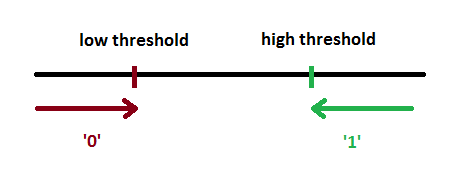
\includegraphics[width=\textwidth]{thresholds}
\newline
Thus we must verify the thresholds are upheld so that for all signals below the low threshold, it is read into the gate as a '0' and produces the correct corresponding output.  This must also be verified for all signals above the high threshold. We first work with a single input and make some assumptions:  1) that passing the signal at the low and high threshold though the gate produces the proper binary output signal, 2) the gate function is a monotonic function.  Then all inputs below the input low threshold or above the input high threshold gives valid output signals as well.  We first assume the function G() is monotonically increasing, the reasoning is thus for all $input low$ $x_i$ pairs, where $input low>x_i$ then $G(input low)>G(x_i)$.  The same could be shown for $input high$ and $x_j$.  If the function G() is monotonically decreasing then the inequality sign of the previous argument is flipped and the correct operation of the circuit still holds.  We verify that our initial assumptions hold in that we can set the output low and high thresholds accordingly, and the Hill function is indeed a monotonic function. 
%there are actually examples where this fails 0->0 in monotonically decreasing... need to fix too
\newline \newline
The next step is when gates are connected to each other, signals must propagate meaningfully as well.  The output of a gate should read as the same binary value into the input of the following gate based on their respective thresholds.  That is for the $i^{th}$ component which is connected to the $i+1^{th}$ component, $output_i low \leq input_{i+1} low$ and $output_i high \geq input_{i+1} high$.  Multiple inputs are common in biology where there can be activators and repressors and even degradation enzymes involved in one gene product.  This is easily reducible to the familiar problem in one dimension.  In biological systems where the ODE model is a sigmoidal curve in the form of a Hill function, the partial derivative with respect to any one input variable is always monotonic.  Thus this satisfies our monotonic requirement and allow for proper propagation. % In addition, because these equations are monotonic with regard to any one variable, there are only a limited number of logic that can be formed.  (expand?)
\newline \newline
The other property that sigmoidal curves are important for is the restorative property of signals to allow for noise and increase robustness.  For the signals to allow a certain amount of noise to enter the system, we would want the output thresholds of one gate to be as far away from the input thresholds of the next gate as possible.  Thus when noise gets added to the output signal, it still has a good chance to transmit the correct binary data to the next stage.  In addition, these components can be connected in a loop.  In electronics, since the outputs and inputs are measured against the same unit of measurement, the voltage, the additional requirement is that the gain must be greater than 1.  This means that the slope of the function should be greater than 1.  Because we are using different chemical species at each stage to transmit the biological signal, we need to scale the slopes of the function accordingly.  
%Sigmoidal, All the things about how they connect, why they are good latches/ memory elements, completion signals?
\newline \newline
Changing rates of degradation of proteins is an important aspect of the circuit that has been often ignored in previous models.  In past papers, gene regulatory networks has been modeled as boolean circuits with each gene/protein element represented by a boolean logic gate.  Each gene logic gate has inputs, usually its activators and repressors, to determine whether the protein is being actively produced or not.  These are usually modeled as AND or OR gates with its promoter binding compounds as its only inputs.  However, in our investigation using the ODE model of each gene, we found that degradation is a crucial part of the logic gates as well.  Protein degradation can be sped up through controlling the production of degradation enzymes.  Meanwhile for stable proteins, it is possible for the base degradation rate, the half life of the protein to be equivalent to the length of the cell cycle, the only reduction in protein concentration coming from the splitting of cells.  These proteins, once produced would remain in the cells for a very long time and essentially considered 'on' even when transcription and/or translation has stopped.  Thus there needs to be a separate way of representing the production of proteins from its degradation.  We take inspiration from Complementary Metal–Oxide–Semiconductor (CMOS) technology.  In CMOS there is a pull up network and a pull down network.  In the inverter example, the pull up network consists of a PMOS and the pull down network consists of a NMOS.  PMOS behaves, on first order approximation, as a conductor when the input voltage is low and as an open switch when the input voltage is high.  NMOS is the opposite, it behaves as an open switch when the input voltage is low and as a conductor when the input voltage is high.  Thus when the input voltage is low, the output voltage is pulled up by the PMOS to a high voltage.  Meanwhile when the input voltage is high, the output voltage is pulled down to ground by the NMOS.  The transcriptional and translational regulation of these genes are similar to a pull up network while the accelerated degradation is similar to a pull down network.  If the background degradation is significantly slower, this effect can be thought of as similar to the parasitic capacitance that slowly leak the charge of the output signal.  Overtime it degrades the output signal however for short time scales the output retains its voltage value and can be considered a dynamic memory element.  Dynamic memory elements are important in asynchronous circuits because they can hold the signal for some time until they receive input, usually from elements further down the circuit to signal that the current output has been acknowledged and processed already and does not need to hold anymore.
\newline \newline
%(write about dynamic memory later?)
\newline
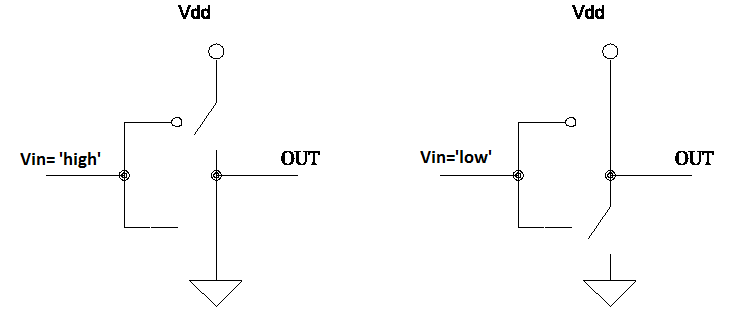
\includegraphics[width=\textwidth]{mosinaction}
\begin{center}
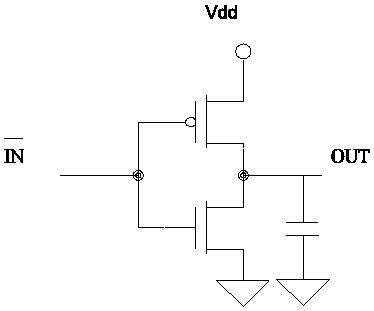
\includegraphics{mosinv}
\end{center}
\section{Static and Dynamic Memory}
There are certain network motifs in biology that allows cells to have some sort of memory.  Our main examples are from Caulobacter but these motifs are present in other cells and thus this analysis is widely applicable.  
%There are positive feedback loops such as in CtrA where once enough production of CtrA starts the feedback, it will remain locked in that high state.  Until degradation overpowers the feedback and pulls CtrA back down to a low state.  This bistable property is also how latches in digital circuits store memory. 
We take inspiration from dynamic memory and look into the short term behavior of each gate.  As mentioned in the previous section, when the degradation term is slow, the changes in protein concentration over time is slow as well.  For very stable proteins, the half life of the protein is then only from splitting of the cells during each cell cycle.  We examine whether using experimentally determined parameters, it is possible to view these gates as memory elements.  For our analysis, we assume that the inputs are held constant.  Then there is a closed form exponential solution of our ODE model.  We can then determine the time elapsed from a given starting state to a final state.  (z is the output protein concentration, and c is the total contribution by the inputs, a constant if the inputs are held constant, $\lambda$ is the degradation rate)
\[\frac{dz}{dt}=c-z\cdot\lambda
\]
The solution to this ODE is the exponential:
\[z(t)=((z_0\cdot\lambda-c)e^{(-\lambda\cdot t)}+c)/\lambda
\]
Where $z_0$ is the inital concentration of the protein.  To find the time elapsed between $z_0$ and some $z_f$ just substitute $z(t)=z_f$.  We also note that at steady state $c=z_{ss}\cdot\lambda$.  Rearranging the equation for time:
\[\Delta t= -log(z_f-z_{ss})/ \lambda+ log(z_0-z_{ss})/ \lambda
\]
 This is the amount of time it takes where $z_0$ is the initial protein concentration and $z_f$ is the final protein concentration.
\newline
%something about robustness?
\begin{center}
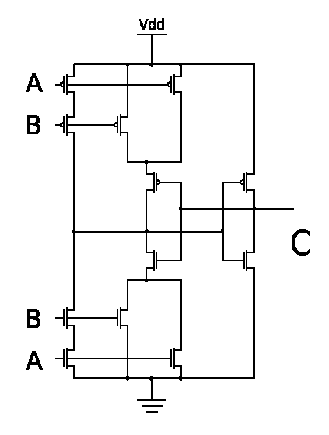
\includegraphics{celement}
\end{center}
The Muller C-element is useful in the design of asynchronous circuits.  If every signal in a circuit is connected with C-elements then it ensures that the circuit can run robustly and has the speed independence property.  Thus we would ideally want the elements we see in biological circuits to operate similarly to the C-element.  A common CMOS implementation of a C-element is shown with two inputs A and B, and an output C.  It operates similarly as the inverter example.  In this C-element example, when A and B are both high, the pull down network is activated, while there are open switches in the pull up network and the output is connected to the ground.  When both A and B are low, the opposite is true and the output is pulled to $V_{cc}$.  However when A and B are different signals ie A is high and B is low or when A is low and B is high, then there is no path through either the pull up or the pull down network and the previous value of the output is retained.  This state is called a 'hold'.
\newline 
\begin{center}
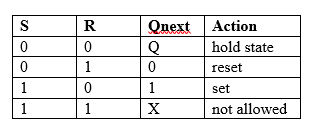
\includegraphics{srlatch}
\end{center}
Set reset latches have a similar modes of operation with output high output low and hold but also differs in an important detail.  In a set reset latch, there are two inputs, called a set and a reset.  We look at the set reset NOR latch.  When set is high and reset is low then the output signal is 'set' or becomes high.  When set is low and reset is high then the output signal is 'reset' or becomes low.  If both inputs are low then the output does not change and is in the hold state.  The last state when both inputs are high gives an undefined output represented by 'X', usually this element does not go into this state.  The similarities between set reset latches and C-elements are quite apparent.  It is basically equivalent if you treat the reset signal of the set reset latch as an inverted second signal for the C-element.  However, when A is high and B is low, there is a hold state for the C-element whereas that corresponds to a high set and high reset and thus an undefined output for the set reset latch.
\newline  \newline
In our model we wish to verify the set reset property of each gene gate.  We use the above equation to check if the time for maximum set or reset transitions is smaller than the time during the hold state.  
Let the input thresholds be:  0 is between $in_{min0}$ and $in_{max0}$ and 1 is between $in_{min1}$ and $in_{max1}$, (the fanout thresholds $fanout_0$ and $fanout_1$ must be between $g(in_{max0})$ and $g(in_{min1})$ )
The maximum time it takes to set or reset in terms of output values is then: \newline
Set- $out_{min0}$ - $fanout_1$ where the input is changed to inmin1 \newline
Reset- $out_{max1}$ - $fanout_0$ where the input is changed to inmax0 \newline
For holds we want the minimum time it stays in output 0 or 1 as the inputs are changed \newline
$out_{max0}$ - $fanout_0$ with max \newline
$out_{min1}$ - $fanout_1$ \newline
\[\Delta t_{set}= - \frac{1}{\lambda} log(g(in_{min1})-fanout_1)/(g(in_{min1}) -g(in_{min0}))
\]
\[\Delta t_{reset}= -\frac{1}{\lambda} log(fanout_0 –g(in_{max0}))/(g(in_{max1}) – g(in_{max0}))
\]
\[\Delta t_{hold0}= -\frac{1}{\lambda} log(z_{ss} -fanout_0)/(z_{ss} -g(in_{max0}))				
\]
\[\Delta t_{hold1}= -\frac{1}{\lambda} log(fanout_1 -z_{ss})/(g(in_{min1}) -z_{ss})
\]
%can expand these equations... how we got to it
Using standard parameter values, it is possible to have the hold times to be longer than the set reset times and so for short periods of time, this element can be considered as a set-reset memory element.  Thus we can abstract these biological motifs as a series of static and dynamic memories connected to each other.

\section{Asynchronous circuits}
One important aspect of asynchronous circuit design is having memory elements.  This is because for a asynchronous circuit to be able to function, it must receive feedback signals from the next stage so that it knows if it needs to hold its current value, or if the next stage has received it's signal and can go to the next stage in processing.

\section{Leakiness}
Interestingly, there are a couple examples even in the Caulobacter cell where if you knockout one of the key components of the core cell cycle proteins that the rest of the cycle still tries to proceed.  For example, experiments where GcrA or CcrM has been deleted should halt the cell cycle since they start the transcription of CtrA and DnaA respectively.  However, it has been shown that after some delay DnaA and CtrA levels accumulate enough such that the cell can enter the next phase of the cycle.  This may be attributed to a base rate of leakiness from their promoters and other stochastic effects.  We analyze the likely causes of this observation.

CtrA has positive self-feedback.  Plotting the solutions of the Hill kinetics and a diagonal line, representing that all CtrA are phosphorylated to CtrAP during this feedback, shows that this causes CtrA to be bistable. (figure \ref{fig:ctrapc})  However if you include leakiness of the promoter, that shifts the curve of CtrAP vs CtrA up such that even in the presence of no CtrAP, there is still some CtrA produced from the base rate.  If the leakiness from the promoter is large enough, it can shift the curve up so much that there is only one stable point of the system, where ctrA is high. (figure \ref{fig:ctrapl}) This would explain why deletion of GcrA and the P1 promoter where GcrA binds to delays the accumulation of CtrA.  In an earlier paper \cite{compgenre} Michaelis-Menton (MM) kinetics was used.  In their model, they also observed a restart of CtrA even when the upstream transcription factor GcrA was not present.  This is because the MM curve produces only one stable equilibrium so CtrA will always go high if given enough time.

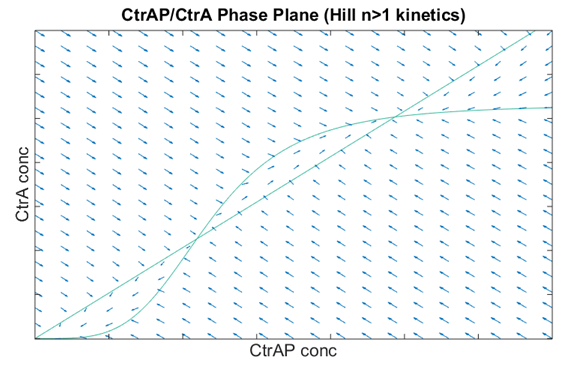
\includegraphics[width=\textwidth]{ctrapc}
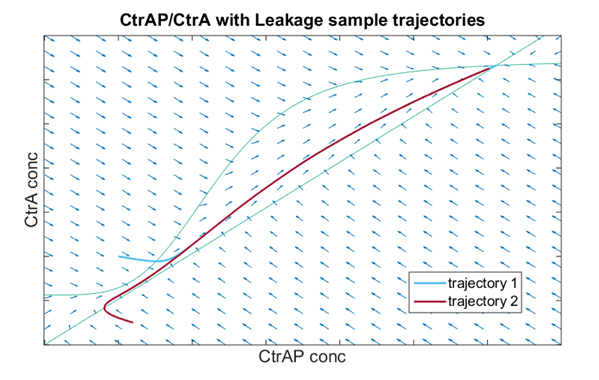
\includegraphics[width=\textwidth]{ctrapl}
\newline \newline
For DnaA, there is evidence that in cells with DnaA lacking the CcrM binding site, the phenotype is not as severe as deleting DnaA directly.  Instead the cell cycle is slowed down.  Thus, there is reason to believe that DnA is also controled by a leaky promoter.  

\begin{thebibliography}{9}
\bibitem{compgenre} 
S M Murray, G Panis, C Fumeaux, P H Viollier , M Howard. 
\textit{Computational and Genetic Reduction of a Cell Cycle to Its Simplest, Primordial Components}. 
PLOS Biology, December 31, 2013.
 
\end{thebibliography}
	
\end{document}
